%%%%%%%%%%%%%%%%%%%%%%%%%%%%%%%%%%%%%%%%%%%%%%%%%%%%%%%%%%%%%%%%%%%%%%%%
% Méthode et résolution
%%%%%%%%%%%%%%%%%%%%%%%%%%%%%%%%%%%%%%%%%%%%%%%%%%%%%%%%%%%%%%%%%%%%%%%%

\section{Environnement de travail}
%=================================

	\subsection{Le Centre de Calcul de l'IN2P3}
	%------------------------------------------

Le centre de calcul de l'IN2P3 (\CC) est une unité de service et de recherche, sont but est de fournir tous les services informatiques demandés par les équipes de recherche de l'IN2P3 regroupées en une trentaine de projets. L'activité du \CC{} est divisée en différents domaines d'expertises :
	\begin{itemize}
		\item Calcul et traitement de données
		\item Stockage
		\item Réseaux et télécoms
		\item Systèmes
		\item Support aux utilisateurs
		\item Systèmes d’information et de communication
		\item Grille informatique
	\end{itemize}
L'aspect du \CC{} utilisé durant ce stage est le calcul et traitement des données. Dans ce domaine, plus de 1\,100 machines biprocesseurs sont accessibles, ce qui correspond à une puissance de calcul de l'ordre de 3.5 TFlops\footnote{TFlops : \emph{tera-flops}, le \emph{flops} (\emph{FLoating-point Operations Per Second}) correspond au nombre d'opérations réalisable par seconde, le préfixe \emph{tera} correspond à $10^{12}$. $3,5$\,TFlops correspond donc à $3,6\cdot 10^{12}$ opérations par seconde.}. Ces machines sont prévues pour le calcul intensif sont aussi appelées machines de \emph{batch}\footnote{\emph{Batch} : anglicisme signifiant « traitement par lot », cela indique que la même tâche sera effectuée sur chaque donnée, sans intervention d'un utilisateur pouvant faire du cas par cas. Une machine de \emph{batch} est une machine prévue pour le calcul et le traitement de masse ; pour cela elle dispose de nombreux cœurs et différents processeurs, ainsi qu'une importante mémoire vive.}, elles sont accessibles depuis des machines d'accueil servant au développement, la compilation, et la mise en place des programmes devant tourner sur les machines de calcul.

\

Une connexion \emph{type} au \CC{} s'effectue ainsi :
	\begin{enumerate}
		\item Connexion SSH aux machines d'accueil via la commande suivante :
		\begin{verbatim}
			$ ssh user@ccage.in2p3.fr
		\end{verbatim}%$
		où \texttt{user} correspond au nom d'utilisateur au \CC{} ;
		\item Développement, compilation du programme ;
		\item Lancement des \emph{jobs} sur les machines de \emph{batch} à l'aide de \texttt{qsub}.
	\end{enumerate}
Ces étapes peuvent être résumées à l'aide du schéma de la figure~\ref{fig:cc-querry}.
	\begin{figure}
		\centering
		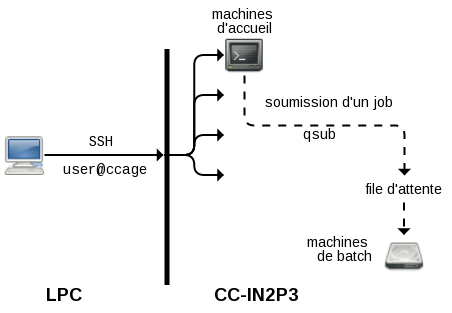
\includegraphics[width=0.9\textwidth]{img/cc-querry.png}
		\caption[Organisation d'une soumission de job au CC-IN2P3]{Organisation des étapes de la soumission d'un job au CC-IN2P3.}
		\label{fig:cc-querry}
	\end{figure}
Une fois envoyé, le \emph{job}, ou programme, agit seul sans interaction possible avec l'utilisateur. Le seul retour à l'utilisateur s'effectue à la fin de l'exécution du programme. Lorsqu'un programme est encore à l'état de développement, l'absence de retour direct à l'utilisateur est une contrainte qui diminue le nombre de tests envisageable. Le fonctionnement de \texttt{qsub} et de la soumission des \emph{jobs} sera expliqué plus en détail dans la partie~\ref{ssec:soumission-jobs}.

	\subsection{Choix des langages}
	%------------------------------

Le projet LSST est entièrement construit sur le couple de langage \Python/\Cpp.

			\paragraph{\Cpp}
Le langage \Cpp{} est un langage compilé, ce qui signifie que le code est d'abord converti en langage machine au cours de la compilation pour former un exécutable propre à une architecture \emph{hardware} pour un système d'exploitation donné. L'intérêt réside dans la vitesse d'exécution, puisque l'exécutable est directement lu par la machine sans le moindre interpréteur.

Le \Cpp{} est un langage relativement bas niveau, cela signifie que la gestion de la mémoire est en bonne partie laissée au programmeur. Cela rend le développement plus long, et nécessite un certain nombre de connaissances pour éviter des erreurs de programmation.

Du fait de sa vitesse d'exécution le \Cpp{} est souvent utilisé pour des moteurs de calcul, ou des tâches sur un grand nombre de données.

			\paragraph{\Python}
Le langage \Python{} est un langage interprété, ce qui signifie qu'au moment de l'exécution, chaque ligne est traduite en langage machine avant d'être exécutée, et ce à chaque exécution d'un même script \Python. Les performances du \Python{} sont jusqu'à 100$\times$ moindre que celles du \Cpp{} comme le montre la figure~\ref{fig:cpp-py}.
	\begin{figure}
		\centering
		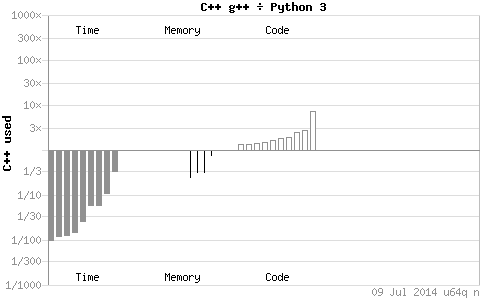
\includegraphics[width=0.8\textwidth]{img/cpp-py.png}
		\caption[\emph{Benchmark} entre \Cpp{} et \Python]{Étude de \emph{benchmark} entre \Cpp{} et \Python{}. Cette étude compare les performances de \Python{} par rapport au \Cpp{} en effectuant le quotient \fraction{Performance \Cpp}{Performance \Python}, donc les résultats en dessous de 1 sont en faveur de \Cpp{}, ceux au dessus de 1 en faveur de \Python{}. Les tests s'effectuent en 3 catégories, temps d'exécution, utilisation de la mémoire et nombre de lignes de code. Chaque barre de l'histogramme dans une catégorie correspond à un algorithme (\emph{n-body}, \emph{mendelbrot}, \emph{binary-trees}, etc.). Source : \url{http://benchmarksgame.alioth.debian.org/}}
		\label{fig:cpp-py}
	\end{figure}
\Python{} est certes moins performant que \Cpp{}, mais il a l'avantage de facilité la programmation avec un nombre de lignes de code moins élevé, des fonctions haut niveau dans la bibliothèque standard et l'interpréteur qui permet un débogage plus rapide. \Python{} est donc privilégié pour la partie interface ainsi que l'ordonnancement des différentes tâches, laissant le cœur du calcul à \Cpp.

			\paragraph{\texttt{Boost}}
\texttt{Boost} est une bibliothèque \Cpp{} qui rajoute de nombreuses fonctionnalités utilisées au quotidien à la bibliothèque standard de \Cpp. \texttt{Boost} est pionnier dans les algorithmes et optimisations en \Cpp, ainsi que dans sa facilité d'écriture. Une partie importante des avancées de \texttt{Boost} est intégrée plus tard dans la bibliothèque standard de \Cpp{}, en servant de base à l'élaboration des nouvelles normes de \Cpp{} comme la norme \Cpp \texttt{1x} \cite{BOOST}.

Cette bibliothèque sera utilisée essentiellement pour la simplicité d'écriture de certaines conversion de données.

			\paragraph{\texttt{ROOT}}
Le \emph{framework} \texttt{ROOT} a été développé au CERN\footnote{CERN : Organisation européenne pour la recherche nucléaire.}, écrit en \Cpp{} et conçu à l'origine pour l'analyse des données en physique des particules. Aux vus de l'historique du LPC, de nombreuses personnes utilisent ce \emph{framework} pour leurs publications, en particulier pour la réalisation de graphiques de qualité. Les standards de LSST n'ont pas encore été définis pour la partie analyse des résultats ; cette partie est pour le moment davantage laissée aux habitudes de programmation de chacun. Les physiciens du LPC travaillent généralement sur des projets annexes en physique des particules pouvant avoir lien avec le LHC\footnote{LHC : (\emph{Large Hadron Collider}) est un accélérateur de particules au CERN.} où le standard est \texttt{ROOT}.

Ainsi \texttt{ROOT} est intégré ici pour la réalisation de graphiques pour garantir une maintenance du code, ainsi que sa lisibilité par les différents physiciens du LPC.

			\paragraph{\emph{R}}
Le langage \emph{R} est un langage interprété prévu pour la réalisation d'études statistiques et de graphiques permettant la visualisation de nombreuses données. C'est un projet GNU\footnote{GNU : (\emph{GNU-s Not Unix}) fait référence ici à la licence libre GNU GPL.} successeur libre du langage \emph{S}. Cet outil fut utilisé dans un premier temps pour la réalisation de tous les graphiques de ce stage ; il fut finalement remplacé par \texttt{ROOT} pour des raisons de performances et de précision des tracés. \emph{R} reste utilisé pour quelques graphiques pour sa simplicité d'écriture.


\section{Comparaison}
%====================

La comparaison s'effectue en 3 étapes ; il est tout d'abord nécessaire de récupérer les données que nous voulons analyser, celles-ci étant disséminées ; nous les rassemblons pour ensuite effectuer la comparaison des deux bases de données. Enfin une étude statistique permet de générer des graphiques pour aider à analyser les résultats de la comparaison. Ces étapes sont lancées sous forme de \emph{jobs} soumis à une machine de \emph{batch} au \CC.

	\subsection{Récupération des données}
	%------------------------------------

La récupération des données s'effectue en deux phases ; tout d'abord la récupération des sources lumineuses identifiées par l'algorithme de SDSS, dont les résultats sont disponibles librement, puis la récupération des sources identifiées par le \stack{} au moment de la \DC.

Nous sauvegarderons ces données au format \texttt{csv} (\emph{comma-separated values}), qui est une organisation de fichiers texte permettant une lecture et une écriture relativement simple. Les données sont séparées par des virgules ou des point-virgules lorsqu'il y a possibilité d'ambiguïté (données numériques respectant la typographie française \cite[p.~124]{IN} ou présence de chaînes de caractères).

	\begin{table}[h]%
		\centering
		\subfloat[Repr\'esentation des donn\'ees]{%
			\input{|"model/csvtolatex.sh table"}
		}%
		\hspace{1em}
		\subfloat[Fichier \texttt{csv} associ\'e]{%
			\input{|"model/csvtolatex.sh csv"}
		}
		\caption[Représentation d'un tableau et du fichier \texttt{csv} associé]{Exemple de la représentation d'un tableau de données et du fichier \texttt{csv} associé.}%
	\end{table}

		\subsubsection{Hiérarchie des données}
		%^^^^^^^^^^^^^^^^^^^^^^^^^^^^^^^^^^^^^

La recherche de ces données est dépendante de la hiérarchie des fichiers, puisque les résultats ne sont pas disponibles directement dans une base de données relationnelle, type SQL, mais dans une foule de fichiers \texttt{fits}, environ 16\,000 paires de fichiers. Une paire de fichiers est consituée :
	\begin{itemize}
		\item D'un fichier \texttt{calexp} contenant l'image calibrée (correction entre autres des erreurs optiques et de l'électronique) ainsi que des informations sur l'astrométrie de l'image (la qualité du fond de ciel, les coordonnées de la région observée, \emph{etc.}).
		\item D'un fichier \texttt{src} contenant un tableau binaire avec la liste des sources, leurs coordonnées astronomiques, leur magnitude, ainsi que diverses informations sur la PSF\footnote{PSF : (\emph{Point Spread Function}) est la fonction d'étalement d'un point et permet de décrire où se situe un objet ponctuel, ici une étoile, à partir de sa réponse dans un système optique, le télescope, avec lequel on observe une tâche.} de la source.
	\end{itemize}
Les deux fichiers de la paire, représentent la même portion de ciel.

\

	\begin{figure}[h]
		\centering
		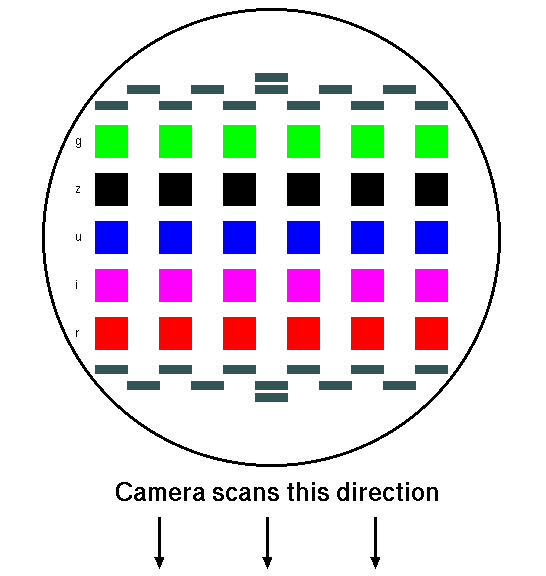
\includegraphics[width=0.6\textwidth]{img/sdss-capteur.png}
		\caption[Schéma du capteur de SDSS]{Schéma du capteur de SDSS ; on y observe les différentes colonnes de CCD dans le sens de la prise de vue, composées de 5 filtres allant de l'ultraviolet à l'infrarouge.}
		\label{fig:sdss-capteur}
	\end{figure}

Ces fichiers sont triés suivant une hiérarchie dépendante de la méthode de prise de vue de SDSS, et de la construction de son capteur, dont une représentation schématique est visible sur la figure~\ref{fig:sdss-capteur}. Les fichiers sont d'abord triés par \emph{run}, ce qui correspond à une mission d'observation, ensuite par colonne. Durant une \emph{run} SDSS se déplace à déclinaison constante, donc tous les capteurs d'une même colonne observeront la même portion de ciel à des instants $t+\Delta t$. Ainsi la même portion de ciel sera visible dans toutes les longueurs d'onde sélectionnées par les filtres. Les fichiers sont ensuite triés par filtre, puis par prise de vue puisqu'une seule \emph{run} correspond à plusieurs photos.

Une image de sortie de SDSS fait $2\,048 \times 1\,361 \mbox{px}^2$ pour un champ correspondant à peu près à celui de la pleine Lune.

\

La hiérarchie des fichiers est rappelée pour chaque fichier par un numéro indiquant la \emph{run} (\texttt{rrrrrr}), le filtre (\texttt{b}), la colonne (\texttt{c}) et le champ observé (\texttt{ffff}), sous la forme suivante :
\begin{verbatim}
	calexp-rrrrrr-bc-ffff.fits
\end{verbatim}
Ce fichier se trouve à l'emplacement : \texttt{rrrrrr/c/b/} où se trouvent tous les fichiers d'une \emph{run}, pour une colonne particulière, pour un filtre précis.

		\subsubsection{Visualisation des données}
		%^^^^^^^^^^^^^^^^^^^^^^^^^^^^^^^^^^^^^^^^

Les données peuvent être visualisées à l'aide du programme \texttt{fv} développé par la NASA (voir figure~\ref{fig:fv}).

	\begin{figure}[h]
	  \centering
	  \subfloat[Image du fichier \texttt{calexp}]{\label{fig:fv-calexp}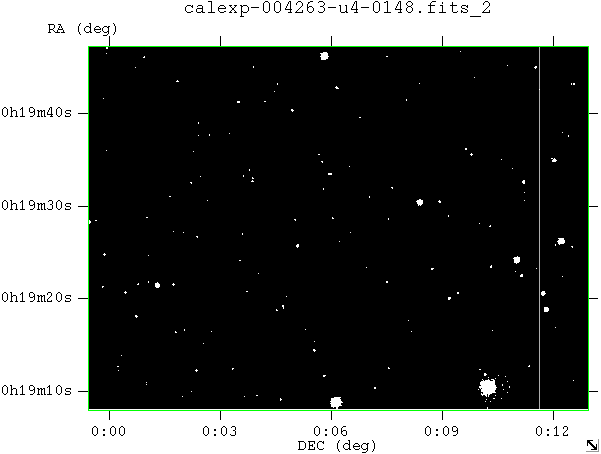
\includegraphics[width=0.45\textwidth]{img/fv-calexp.png}}
	  \hspace{5pt}
	  \subfloat[Table binaire du fichier \texttt{src}]{\label{fig:fv-src}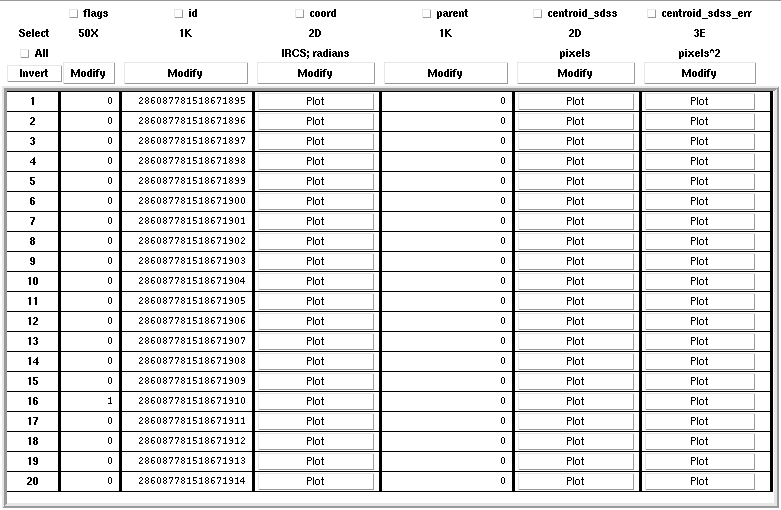
\includegraphics[width=0.45\textwidth]{img/fv-src.png}}
	  \\
	  \subfloat[Graphique des sources du fichier \texttt{src}]{\label{fig:fv-src-pict}\includegraphics[width=0.45\textwidth]{img/fv-src-pict.png}}
	  \caption[Visualisation des données avec \texttt{fv}]{Visualisation des fichiers \texttt{calexp} et \texttt{src} à l'aide du logiciel \texttt{fv}. Le fichier \texttt{calexp} contient une image du ciel calibrée et corrigée, le fichier \texttt{src} contient un tableau des sources identifiées par le \stack ; le logiciel \texttt{fv} permet de plus de placer les sources identifiées dans la table binaire dans le plan.}
	  \label{fig:fv}
	\end{figure}

		\subsubsection{Les données SDSS}
		%^^^^^^^^^^^^^^^^^^^^^^^^^^^^^^^

On remarque avec la figure~\ref{fig:fv} que les données de SDSS ne sont pas présentes dans les fichiers stockés au \CC{}, ces données sont accessibles sur une base de données accessible via l'Internet. Une interface permet l'écriture de requêtes SQL directement soumises sur ce site : \url{http://cas.sdss.org/stripe82/en/tools/search/sql.asp} [Online ; accès : 2014-07-10]. Le schéma de construction des tables SQL est aussi disponible sur le site de SDSS\footnote{Les schémas des tables SQL sont disponibles à l'adresse suivante : \url{http://cas.sdss.org/stripe82/en/help/browser/browser.asp} [Online ; accès : 2014-07-10].}. Pour simplifier la récupération automatique des données, indispensable pour du traitement par lots, un script \Python{} est fourni par l'équipe de SDSS\footnote{Le script de requête automatique est disponible sur \url{http://cas.sdss.org/stripe82/en/help/download/sqlcl/} [Online ; accès : 2014-07-10].} mais une modification du script est nécessaire pour cibler non pas la dernière mise à jour de la base de données globale de SDSS (\emph{data release 7}) mais seulement les données de la \emph{stripe 82}.

\

La base de données de SDSS est soumise à des restrictions pour permettre un accès continu à tous. Ainsi la taille des requêtes est limitée, ainsi que le nombre de requêtes par minute. Pour pallier ces limitations, une copie de la base de données existe et a été téléchargée au LIMOS\footnote{LIMOS : Laboratoire d’Informatique, de Modélisation et d’Optimisation des Systèmes.} pour le projet \emph{PetaSky} qui est un projet plus spécifique à la gestion de la base de données et aux problèmes de \emph{Big-Data} engendrés par LSST. Cette base au format Microsoft SQL Server ne peut, pour un problème de licence, être chargée au LPC. L'accès à la base de données au LIMOS, ou sa conversion au format libre MySQL ayant pris du retard, l'accès aux données s'effectue pour le moment toujours par le biais des serveurs de SDSS.

\

Finalement, pour garantir un accès constant aux données de SDSS nécessaire à la comparaison, toutes les données ont été récupérées au format \texttt{csv}. Cette méthode ne peut être envisagée pour le passage à l'échelle, c'est à dire la totalité des résultats de la \DC{}, pour des raisons de volume. La mise en base de ces données dans une base de données MySQL fut envisagée sur la fin du stage. Cette base en plus de contenir les données de SDSS et du \stack{}, a vocation à contenir les résultats des différents algorithmes de comparaisons pouvant par la suite servir de pilier fondateur d'un catalogue.


		\subsubsection{Les données LSST}
		%^^^^^^^^^^^^^^^^^^^^^^^^^^^^^^^

L'accès aux données générées par la \stack{} est plus simple comme le montre la figure~\ref{fig:fv}\subref{fig:fv-calexp}. En effet le fichier \texttt{src-rrrrrr-bc-ffff.fits} contient directement les données qui nous intéressent, c'est-à-dire les coordonnées (ascension droite et déclinaison) ainsi que la magnitude relative à l'image. Il est cependant nécessaire de recalibrer la magnitude à l'aide d'une donnée disponible dans une base de données, indiquant une valeur de calibration pour chaque fichier.




		\subsubsection{Algorithme de principe}
		%^^^^^^^^^^^^^^^^^^^^^^^^^^^^^^^^^^^^^

Le module de recherche des données est entièrement écrit en \Python{}, cela permet en quelques lignes de récupérer les données nécessaires à la comparaison des deux jeux de données.

L'UML\footnote{UML : (\emph{Unified Modeling Language}) langage graphique de modélisation.} permet schématiquement de représenter, à l'aide d'un diagramme d'activité, les différentes étapes nécessaires à la récupération des données. Le diagramme d'activité présenté dans la figure~\ref{fig:dia-data} ne respecte pas exactement la norme UML pour pouvoir indiquer plus d'informations concernant les dépendances à certaines données, comme la valeur d'étalonnage \texttt{fluxMag0} qui permet de calibrer la magnitude, ou la recherche à une base de données distance.
\begin{figure}[h]
	\centering
	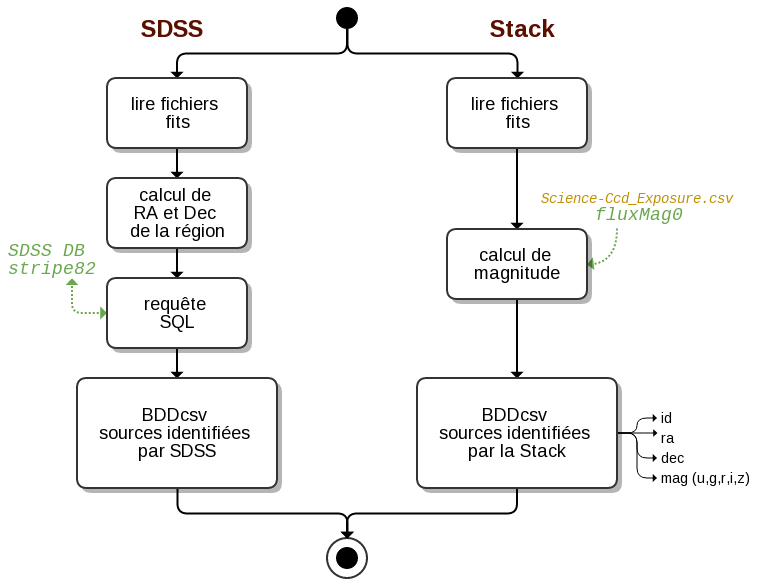
\includegraphics[width=0.9\textwidth]{img/dia-data.png}
	\caption[Diagramme UML d'activité de recherche des données]{Diagramme UML d'activité de recherche des données, avec l'ajout des dépendances tierces.}
	\label{fig:dia-data}
\end{figure}

Ce diagramme représente environ 400 lignes de code commenté, dont voici un exemple pour montrer la simplicité du \Python. Le code~\ref{code:readFits} lit un fichier \texttt{fits} \texttt{src}, il présente la définition d'une fonction \texttt{readFits} prenant comme paramètre le nom du fichier \texttt{fits} à lire, s'en suit la récupération du tableau qui permet de lire toutes les coordonnées dans la colonne/champ \texttt{coord}.

	\lstinputlisting[language=Python, caption={Lecture d'un fichier \texttt{fits} en \Python}, label= {code:readFits}]{code/readFits.py}

	\subsection{Comparaison}
	%-----------------------

Les données récupérées au format \texttt{csv} au cours de la récupération des données sont analysées dans un module écrit en \Cpp{}. À l'origine ce module fut écrit en \Python, mais pour des questions de performance il a été remplacé par du \Cpp{}. En effet, en moyenne le script en \Python{} s'exécutait en 1\,min et 20\,s, le passage au \Cpp{}, sur le même jeu de données a fait descendre ce temps d'exécution à 0,13\,s. En revanche le temps de développement est passé d'une demi-journée (74 lignes de code), à 4 jours (756 lignes de code) ; on voit ici la vraie force de \Python{} qui est sa simplicité d'écriture à l'aide de nombreuses fonctions haut-niveau.

\

Pour comparer les deux bases de données, il est tout d'abord nécessaire d'effectuer une association des sources SDSS avec les sources du \stack. Différents algorithmes, sont envisageables ; en effet cela se traduit souvent par une recherche de plus proche voisin ; certaines méthodes permettent d'introduire, en plus des paramètres astrométriques, des paramètres photométriques, plus sensibles à l'erreur, comme la magnitude, qui permettent d'associer uniquement des sources lumineuses d'intensité semblable, donc plus susceptibles de faire référence à la même source.

		\subsubsection{Association à voisinage constant}
		%^^^^^^^^^^^^^^^^^^^^^^^^^^^^^^^^^^^^^^^^^^^^^^^

La première méthode implémentée considère que deux sources, une identifiée par SDSS et une par le \stack, sont identiques si elles sont à moins de $2"$\footnote{$2"$ : 2 arc-seconde, une seconde d'arc correspondant à \fraction{1}{3\,600}\up{e} de degré.}, ce qui correspond au diamètre apparent de Mars. Si plusieurs sources sont identifiées dans cette fenêtre de $2"$ alors on compare leur magnitude. Cette méthode peut être appelée une comparaison à $\epsilon$ près avec $\epsilon = 2"$.

Un algorithme de principe est décrit dans l'algorithme~\ref{algo:cmp-vois} avec la structure de données décrite schématiquement dans la figure~\ref{fig:sdd-vois}. L'algorithme est globalement en $\mathcal{O}(n^2)$ puisqu'il s'agit d'une boucle sur tous les éléments d'une liste à l'intérieur d'une boucle sur tous les éléments d'une même liste. Idéalement ces deux listes ont le même nombre d'éléments $n$. La gestion des erreurs oblige à effectuer des boucles supplémentaires, par exemple au moment de l'ajout d'un élément dans une liste triée, la vérification qu'une source n'est pas associée plusieurs fois ou qu'elle n'est pas oubliée.
	\begin{algorithm}
		\caption{Association à voisinage constant}
		\label{algo:cmp-vois}
		\begin{algorithmic}[1]
			\ForAll{Source SDSS}
				\State Initialisation de $listSDSS$; \Comment{Liste des sources associées à la source SDSS courante}
				\ForAll{Source Stack}
					\If{ $Distance(SDSS ; Stack) \leq \epsilon$ }
						\State Ajout de la source Stack dans $listSDSS$;
						\Comment{listSDSS est triée par $|\Delta mag|$ croissant}
					\Else
						\State Passer à l'élement suivant;
					\EndIf
				\EndFor

				\State Sélection du premier élément de $listSDSS$ pour la source SDSS courante;

			\EndFor

			\State Vérification de l'unicité des choix de sources, gestion des erreurs;
		\end{algorithmic}
	\end{algorithm}

	\begin{figure}[h]
		\centering
		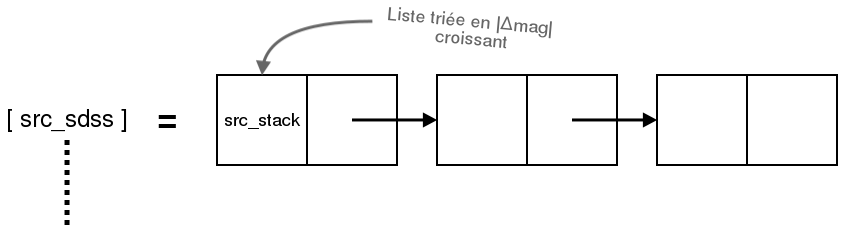
\includegraphics[width=0.8\textwidth]{img/sdd-mapsrc.png}
		\caption[Structure de données de la comparaison à voisinage constant]{Structure de données de l'algorithme de comparaison à voisinage constant, une liste chaînée de sources du \stack{} est associée à chaque source SDSS.}
		\label{fig:sdd-vois}
	\end{figure}

La structure de données choisie est un tableau associatif pointant des listes chaînées. Celle-ci fut choisie pour conserver une trace des sources présentes dans une fenêtre de $2"$ autour d'une source identifiée par SDSS. Par la suite cette information ne fut pas conservée mais gardée en cas de besoin d'évolution. En effet s'il est nécessaire d'effectuer la sélection par un autre critère que la magnitude au sein de la fenêtre, un simple tri sur cette liste chaînée le permet.

Cette structure n'est certes pas la plus optimisée mais elle est une des plus lisibles et compréhensibles et permet de conserver le maximum d'information de chaque itération. Ainsi elle fut conservée car le temps de calcul restait raisonnable.

		\subsubsection{Association par plus proche voisin}
		%^^^^^^^^^^^^^^^^^^^^^^^^^^^^^^^^^^^^^^^^^^^^^^^^^

Il est possible d'effectuer l'association sans prendre en compte des paramètres dits "photométriques" comme la magnitude, mais seulement les paramètres "astrométriques" donc les coordonnées mesurées d'une source. Pour cela il suffit d'effectuer une recherche de plus proche voisin.

Un tel algorithme fut expérimenté par D\up{r} Philippe Gris pour une comparaison des différents résultats du \stack{} entre les États-Unis et la France. Il s'agit de minimiser les écarts entre l'association des sources, il est donc nécessaire de calculer tous les $\Delta$ de coordonnées entre les deux jeux de sources, puis de sélectionner un à un les plus faibles différences de coordonnées.

Un tel algorithme sélectionne les plus faibles différences de coordonnées en premier et élimine ces sources de la liste des sources à associer. La complexité de l'algorithme est en $\mathcal{O}(n^2)$.

\

L'association par plus proche voisin peut s'effectuer avec des algorithmes plus perfectionnés comme le \emph{kd-tree} ou l'\emph{quadtree} permettant la diminution de la complexité, avec une complexité sub-linéaire. Ces algorithmes utilisent, comme leur nom l'indique, des arbres pour effectuer cette recherche et effectuent tout d'abord un partitionnement de l'espace qui est l'étape la plus couteuse algorithmiquement. Ce partitionnement permet d'obtenir une notion de voisinage variable.

		\subsubsection{Association par voisinage variable}
		%^^^^^^^^^^^^^^^^^^^^^^^^^^^^^^^^^^^^^^^^^^^^^^^^^

Les algorithmes avancés de recherche de plus proche voisin utilisent un arbre. L'arbre se construit en divisant l'espace de manière récursive. Ici l'espace est la sphère céleste qui sera approximée par un plan.

			\paragraph{\emph{Quadtree}}
Le \emph{quadtree} permet d'obtenir un arbre dont chaque élément a zéro ou quatre fils. Pour cela l'espace est divisé en 4 tant qu'il n'y a pas zéro ou un élément (source lumineuse dans notre cas) dedans. L'algorithme~\ref{algo:quadtree} présente la version récursive en supposant que les fonctions retournant les quatre quadrants de l'espace sont déjà définies. La dérécursification de l'algorithme ne fut pas envisagé car apportant trop peu de chose. Cet arbre fut abandonné car l'arbre n'est pas équilibré et possède une profondeur trop importante. Ce type d'arbre peut être intéressant lorsqu'il est régulièrement nécessaire de recalculer l'arbre car sa structure est plus évolutive que le \emph{kd-tree}.

	\begin{algorithm}
		\caption{Algorithme récursif de construction du \emph{quadtree}}
		\label{algo:quadtree}
		\begin{algorithmic}[1]
			\Function{DiviseEspace}{$space$}
				\If{ Nb sources = 0}
					\Comment{L'espace ne contient pas de sources}
					\State \Return $space$;
				\ElsIf{Nb sources = 1}
					\Comment{L'espace ne contient qu'une source}
					\State \Return $space$;
				\Else
					\Comment{Il faut diviser l'espace en 4 quadrants}
					\State $space1$ $\gets$ \Call{PremierQuadrant}{$space$};
					\State $space2$ $\gets$ \Call{DeuxièmeQuadrant}{$space$};
					\State $space3$ $\gets$ \Call{TroisièmeQuadrant}{$space$};
					\State $space4$ $\gets$ \Call{QuatrièmeQuadrant}{$space$};
					\State \Return \Call{DiviseEspace}{$space1$}, \Call{DiviseEspace}{$space2$}, \Call{DiviseEspace}{$space3$}, \Call{DiviseEspace}{$space4$}
				\EndIf
			\EndFunction
		\end{algorithmic}
	\end{algorithm}

	\begin{figure}[h]
		\centering
		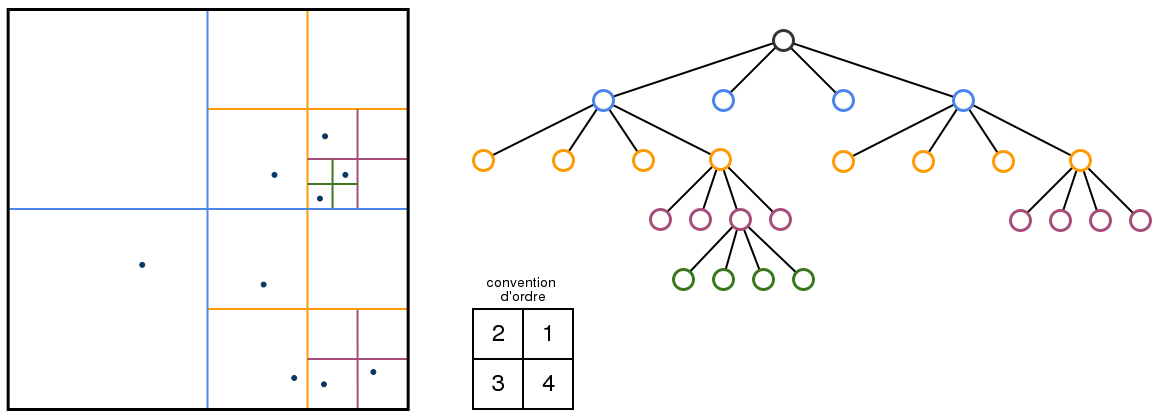
\includegraphics[width=0.9\textwidth]{img/quadtree.png}
		\caption[Relation entre la géométrie de l'ensemble et le \emph{quadtree} généré]{Relation entre la géométrie de l'ensemble (le placement des points dans l'espace), et la structure de données générée, le \emph{quadtree}. Chaque découpage est effectué avec une couleur différente pour voir son association avec l'arbre. La convention d'ordre des fils est celle des quadrants d'un repère orthonormé. On observe le découpage des sous-espaces tant qu'il n'y a pas zéro ou un élément.}
		\label{fig:quadtree}
	\end{figure}

La figure \ref{fig:quadtree} explique graphiquement comment à partir de points sur un plan il est possible de construire un arbre. Cette structure a l'inconvénient d'avoir une profondeur très importante si deux points sont relativement proches ; en effet l'algorithme continuera à diviser l'espace en 4 parts égales tant que nécessaire. Pour éviter ce type de problème, il est possible d'imposer une profondeur maximale à l'arbre généré pour obtenir un premier partitionnement, puis effectuer une association avec un autre type d'algorithme en prenant en compte d'autres paramètres que les coordonnées.

				\paragraph{\emph{kd-tree}}
Un \emph{kd-tree} pour \emph{$k$-dimensional tree}\footnote{Le \emph{kd-tree} comme le \emph{quadtree} est généralisable en dimension $k$ pour des données présentes dans l'espace ou un hyper-espace.} est un partitionnement de l'espace permettant d'obtenir un arbre équilibré. Cela permet d'avoir une meilleure complexité dans le pire des cas qui est de l'ordre de $\mathcal{O}(n \log^2 n)$ si l'algorithme de calcul de médiane a une complexité en $\mathcal{O}(n\log n)$.

Pour obtenir un arbre équilibré, le partitionnement ne s'effectue pas en fonction des caractères géométriques de l'espace (les dimensions), mais en fonction du nombre d'éléments contenus dans celui-ci pour diviser l'espace en deux sous-espaces contenant le même nombre d'éléments à l'aide de la médiane. L'espace étant divisé, tant que nécessaire, en 2 à chaque itération $i$, le calcul de la médiane s'effectue selon une dimension différente entre $i$ et $i+1$.


L'algorithme~\ref{algo:kdtree} permet de présenter la construction d'un \emph{kd-tree}. L'algorithme permettant de trouver la médiane n'est pas détaillé ici, de même que les fonctions divisant l'espace en deux avant et après la médiane.
	\begin{algorithm}
		\caption{Algorithme récursif de construction du \emph{kd-tree}}
		\label{algo:kdtree}
		\begin{algorithmic}[1]
			\Function{kdtree}{$space$,$profondeur$}
				\If{ Nb sources $\leq 1$}
					\Comment{L'espace n'est pas divisable}
					\State \Return $space$;
				\Else
					\Comment{Il faut diviser l'espace en 2 suivant la médiane}
					\If{$profondeur \equiv 0 [2]$}
						\State axe $\gets$ $x$;
					\Else
						\State axe $\gets$ $y$;
					\EndIf
					\State $space1$ $\gets$ \Call{AvantMediane}{$space$, axe};
					\State $space2$ $\gets$ \Call{AprèsMediane}{$space$, axe};

					\State \Return \Call{kdtree}{$space1$, $profondeur + 1$}, \Call{kdtree}{$space2$, $profondeur + 1$}
				\EndIf
			\EndFunction
		\end{algorithmic}
	\end{algorithm}
	\begin{figure}[h]
		\centering
		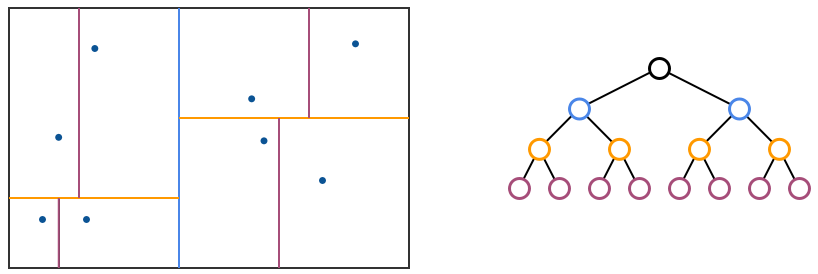
\includegraphics[width=0.9\textwidth]{img/kdtree.png}
		\caption[Relation entre la géométrie de l'ensemble et le \emph{kd-tree} généré]{Relation entre la géométrie de l'ensemble (le placement des points dans l'espace), et la structure de données générée, le \emph{kd-tree}. On remarque très facilement que l'arbre binaire est toujours équilibré grâce au découpage suivant la médiane.}
		\label{fig:kdtree}
	\end{figure}

\

Ces algorithmes permettent la construction d'un partitionnement de l'espace ; la recherche de plus proche voisin dans l'arbre est ensuite une recherche de quelques éléments dans l'arbre, puis s'ensuit un calcul de distance sur un nombre très réduit d'éléments.

Le choix d'un tel type d'algorithme est dû à sa modularité. En effet cette technique permet de construire un voisinage de chaque source dépendant de l'écart entre les sources. Ainsi, après la construction de l'arbre, on ne cherche pas forcément à calculer une distance, mais on peut affiner la recherche avec des paramètres photométriques parmi les sources voisines.

\

La comparaison effectue en réalité une association entre une source de la base de données de SDSS avec une source identifiée par le \stack{}, l'écart de coordonnées et de magnitude est calculé puis sauvegardé au format \texttt{csv}. Les identifiants de SDSS et du \stack{} étant sauvés, une fois l'association effectuée avec différents algorithmes il serait possible d'effectuer une comparaison des résultats.

\

Il a été envisagé d'effectuer un premier test sur un jeu d'essai et de trier les résultats du test en vrai positif, faux positif, faux négatif et vrai négatif. Cette mesure statistique permet d'évaluer la sensibilité d'un test pour catégoriser des évènements. Ce test est en attente de l'implémentation des autres algorithmes d'association, pour le moment seule l'association à voisinage constant est utilisée.


	\subsection{Statistiques}
	%------------------------

La partie statistique est essentiellement un retour graphique des résultats ; en effet l'étape précédente de comparaison s'effectue sur plusieurs milliers de sources, et les fichiers \texttt{csv} de sortie ne permettent pas une analyse directe. Le collectif des physiciens des particules utilise principalement le \emph{framework} \texttt{ROOT} pour les réalisations de courbes, d'histogrammes et de graphes, ainsi que le calcul de données statistiques. En effet le milieu de la physique corpusculaire expérimentale est basé sur des études statistiques d'un grand nombre de données, par exemple l'expérience LHC génère 25 \Po{} de données brutes par an qu'il est nécessaire d'analyser à l'aide d'outils probabilistes et statistiques. \texttt{ROOT} fut développé au CERN pour les besoins de l'époque, et a ensuite évolué vers le \emph{framework} \Cpp{} qu'il est aujourd'hui.

\texttt{ROOT} permet la réalisation de simulations de type Monte-Carlo, il implémente de nombreux algorithmes d'algèbre linéaire, ainsi que des bases de calcul formel comme la dérivation. \texttt{ROOT} simplifie aussi l'interface avec d'autres bibliothèques ; par exemple il permet l'accès à des bases MySQL, ainsi que la lecture de fichiers \texttt{fits}. Cette dernière possibilité ne fut pas exploitée au cours de ce stage malgré la nécessité d'une telle option à cause de la forte présence de bugs dans ce module, ainsi que l'obligation d'un typage fort sans connaissance des types des données utilisées dans le fichiers \texttt{fits}.

		\subsubsection{En \texttt{ROOT}}
		%^^^^^^^^^^^^^^^^^^^^^^^^^^^^^^^

\texttt{ROOT} ne fut utilisé ici que pour la réalisation de graphiques ; ceux-ci peuvent être exportés en tant qu'image au format \texttt{png} ou sous forme d'animation au format \texttt{gif}. Il est également possible d'exporter les données dans un format propre au \emph{framework}. Celui-ci est génère un fichier binaire ouvrable avec l'interpréteur \emph{CINT}. Le graphe est modifiable via une interface graphique et permet de personnaliser l'échelle du repère après l'exécution de la majorité des calculs, et ne pas devoir les relancer pour des modifications esthétiques.

\

\emph{CINT} est un interpréteur \emph{C}/\Cpp{} prévu pour le développement d'algorithmes avec \texttt{ROOT}. Il se présente sous la forme de paquet installé au même moment que \texttt{ROOT}. Son intérêt n'est que le développement et le test d'algorithmes utilisant cet outil, les performances de \emph{CINT} étant plus mauvaises que celles de \Python{} comme le montre le comparatif de \emph{CINT} avec \Cpp{} sur la figure~\ref{fig:cpp-cint}. Pour rappel la comparaison de \Cpp{} avec \Python{} est disponible sur la figure~\ref{fig:cpp-py} à la page~\pageref{fig:cpp-py}.

	\begin{figure}[h]
		\centering
		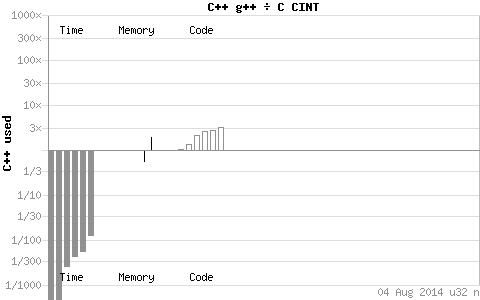
\includegraphics[width=0.8\textwidth]{img/cpp-cint.png}
		\caption[\emph{Benchmark} entre \Cpp{} et \emph{CINT}]{Étude de \emph{benchmark} entre \Cpp{} et \emph{CINT}. Cette étude compare les performances de \emph{CINT} par rapport au \Cpp{} en effectuant le quotient \fraction{Performance \Cpp}{Performance \emph{CINT}}, donc les résultats en dessous de 1 sont en faveur de \Cpp{}, ceux au dessus de 1 en faveur de \emph{CINT}. Source : \url{http://benchmarksgame.alioth.debian.org/}}
		\label{fig:cpp-cint}
	\end{figure}

	\lstinputlisting[language=C++, caption={Création d'un histogramme en \texttt{ROOT} (exemple tiré de la documentation)}, label= {code:root}]{code/fitexample.C}

	\begin{figure}[h]
		\centering
		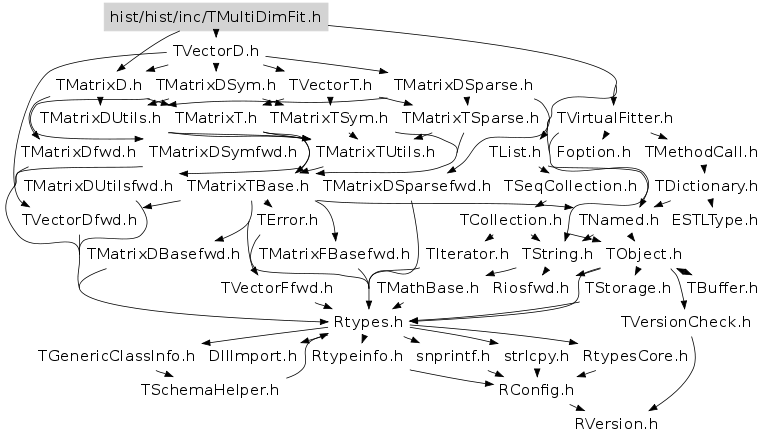
\includegraphics[width=0.8\textwidth]{img/linkroot.png}
		\caption[Lien entre les définitions de classes dans \texttt{ROOT}]{Lien entre les différents entêtes de définition de classe en \texttt{ROOT}. Source \url{http://root.cern.ch/root/htmldoc/}}
		\label{fig:linkroot}
	\end{figure}

\
\texttt{ROOT} présente l'avantage de pouvoir se compiler, cela permet un gain de temps significatif. Mais l'un des problèmes de ce \emph{framework} est la prise en main relativement longue due à une documentation composée d'une suite d'exemples sans pas à pas comme le montre l'extrait de code~\ref{code:root}. La syntaxe imposée par \texttt{ROOT} n'est pas la plus intuitive alors qu'elle pourrait l'être en surchargeant efficacement des opérateurs ainsi que des méthodes. De plus les classes disponibles pour l'utilisateur sont très spécifiques à certaines utilisations et possèdent une hiérarchie non triviale comme le montre la figure~\ref{fig:linkroot}. Malgré tout, \texttt{ROOT} permet des tracés de courbes de précision, avec la présence de barres d'erreurs, des calculs de données statistiques automatiques. Le langage \emph{R} fut choisi dans un premier temps pour sa simplicité d'écriture et sa prise en main rapide, mais le manque de précision de certains calculs ainsi que le temps mis à les effectuer ont joué en faveur de \texttt{ROOT} ; de plus \emph{R} n'étant pas installé au \CC{}, les tracés de courbes devaient s'effectuer en local.

		\subsubsection{Choix des représentations}
		%^^^^^^^^^^^^^^^^^^^^^^^^^^^^^^^^^^^^^^^^

Il existe plusieurs manières de représenter des mêmes données. Par exemple les résultats d'un sondage peuvent être représentés sous forme de diagrammes circulaires, en toiles d'araignée ou d'histogrammes. Chaque culture professionnelle a ses habitudes.

Dans un premier temps il a été envisagé de tracer des boîtes à moustaches, qui permettent de visualiser en une seule fois la moyenne, les quartiles ainsi que les déciles d'un échantillon. Mais le corps des physiciens n'étant pas habitué à ce genre de représentation, le choix définitif se fixa sur des histogrammes. Le tracé de la densité de probabilité fut envisagé, mais le lissage de la courbe empêchait de visualiser des valeurs extrêmes.

\

Le choix d'une représentation dépend du corps de métier mais aussi de l'attente des résultats. En effet dans notre cas, on s'attend à avoir des écarts de coordonnées relativement faibles, donc un pic central proche de zéro très important ; il est donc intéressant de forcer les valeurs isolées à l'aide d'une échelle logarithmique pour voir où a lieu un possible dysfonctionnement de l'algorithme du \stack{}. Le lissage d'une courbe écrase les petites valeurs extrêmes, n'est pas une bonne chose pour quantifier une erreur.

\

Le module de statistique permet à l'aide du \emph{framework} \texttt{ROOT} de réaliser un histogramme de l'écart de magnitude, ainsi qu'un histogramme en 3D de l'écart des coordonnées. Ce dernier est représenté vu de dessus avec un code couleur pour la densité d'évènements, un exemple est visible sur la figure~\ref{fig:histroot}.

	\begin{figure}[h]
		\centering
		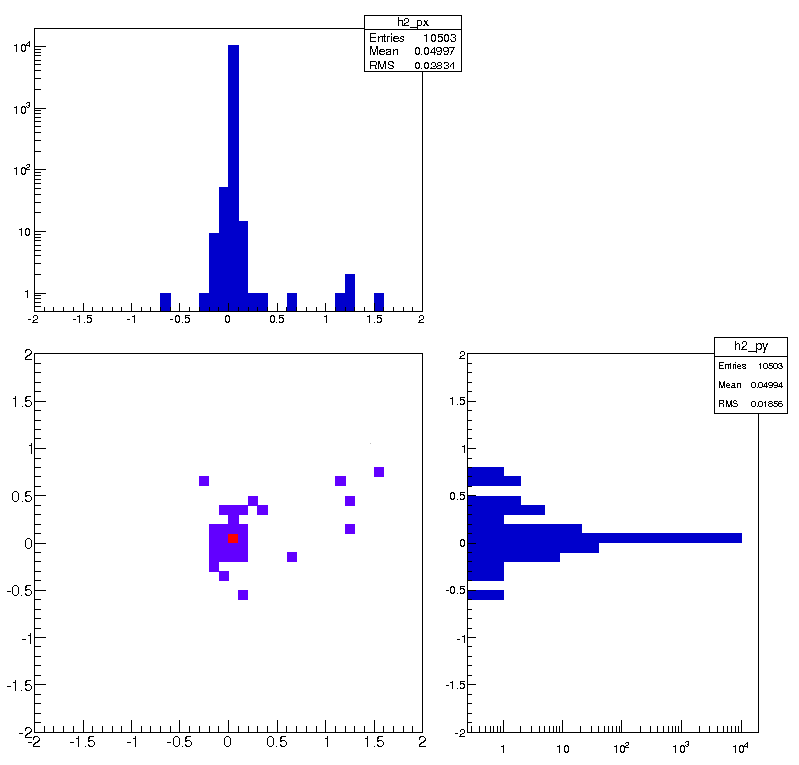
\includegraphics[width=0.8\textwidth]{img/histroot.png}
		\caption[Densité d'écart de coordonnées]{Densité d'écart de coordonnées entre SDSS et le \stack{} sur une \emph{run} en ascension droite (l'axe des $x$) et déclinaison (l'axe des $y$), l'écart est relatif à SDSS : $\Delta X = X_{SDSS} - X_{Stack}$. On remarque l'efficacité du \emph{framework} \texttt{ROOT} qui affiche automatiquement sur un histogramme le nombre d'évènements, la moyenne ainsi que la moyenne quadratique (RMS).}
		\label{fig:histroot}
	\end{figure}


	\subsection{Soumission des \emph{jobs}}
	%--------------------------------------
	\label{ssec:soumission-jobs}

Les données à traiter ne sont disponibles qu'au centre de calcul de l'IN2P3, il est donc nécessaire d'y travailler à distance. Comme le montre la figure~\ref{fig:cc-querry} à la page~\pageref{fig:cc-querry}, on peut soit faire tourner ses programmes sur les machines d'accueil, soit sur des machines de \emph{batch} pour du calcul à plus haute performance, et ne nécessitant pas d'interaction avec l'utilisateur. Pour cela l'utilisateur passe par un ordonnanceur\footnote{Dans le milieu informatique l'anglicisme \emph{scheduleur} est plus usité que le mot français "ordonnanceur".} à qui l'on soumet un \emph{job}, ce dernier entre alors dans une file d'attente avec un système de priorité. L'ordonnanceur définit l'ordre d'exécution des \emph{jobs} qui lui sont soumis par tous les utilisateurs.

L'utilisateur de l'ordonnanceur n'a aucun contrôle sur l'exécution de son programme, celui-ci peut aussi bien être exécuté dès sa soumission, ou plus tard en fonction de l'affluence sur les machines de \emph{batch}. Cela entraîne une période de latence pendant laquelle le programme attend son exécution.

L'ordonnanceur utilisé au \CC{} est \texttt{qsub}.


		\subsubsection{Parallélisation des calculs}
		%^^^^^^^^^^^^^^^^^^^^^^^^^^^^^^^^^^^^^^^^^^

La parallélisation des calculs s'est développée dans les années 2000 où il n'était plus possible d'augmenter sans cesse la fréquence des processeurs pour diminuer le temps d'exécution. Le premier processeur multi-c\oe{}ur commercialisé est POWER4 en 2001 par IBM\footnote{IBM : (\emph{International Business Machines}) est une société multinationale américaine présente dans les domaines de la construction informatique, du développement logiciel et du service informatique.} et marque le début de la multiplication des c\oe{}urs dans les unités de calcul.

La parallélisation permet à un programme de ne pas s'exécuter suivant un seul fil\footnote{L'utilisation du mot "fil" n'est pas anodine puisqu'on parle de \emph{thread} d'exécution, le mot \emph{thread} signifiant "fil".} d'exécution, mais en parallèle sur plusieurs. Le programme peut exécuter plusieurs tâches simultanément si elles sont indépendantes. Un exemple simple de parallélisation est un programme devant ajouter $n$ à tous les éléments d'un tableau. Pour ce faire il suffit d'effectuer une boucle sur tous les éléments du tableau et de leur ajouter le nombre $n$ comme le montre l'algorithme~\ref{algo:boucletab}.

	\begin{algorithm}
		\caption{Parcours d'un tableau en séquentiel}
		\label{algo:boucletab}
		\begin{algorithmic}[1]
			\Function{Parcours\_tab}{$tableau$, $n$}
				\ForAll{$elm$ de $tableau$}
					\State $elm$ $\gets$ $elm+n$;\label{line:boucletab:get}
				\EndFor
			\EndFunction
		\end{algorithmic}
	\end{algorithm}

Imaginons que le temps d'exécution de l'instruction à la ligne~\ref{line:boucletab:get} de l'algorithme~\ref{algo:boucletab} prend $1\,s$, le temps d'exécution de la boucle sera égal au nombre d'éléments du tableau~$\times~1\,s$.

Dans cet exemple la $i$\up{e} itération de la boucle est indépendante de l'itération $i+1$, elles peuvent donc s'exécuter indépendamment l'une de l'autre sur une autre unité logique de calcul. Ainsi la parallélisation de l'algorithme~\ref{algo:boucletab} pourrait se représenter comme suit dans l'algorithme~\ref{algo:paraltab}. La ligne \ref{line:paraltab:ab} effectue le même traitement que la ligne~\ref{line:boucletab:get} de l'algorithme~\ref{algo:boucletab}, le temps d'exécution est le même. Mais dans le cas de l'algorithme de parcours en parallèle, il faut imaginer que chaque appel à la fonction \textsc{Additionne} à la ligne~\ref{line:paraltab:calladd} s'effectue en parallèle. Les fils d'exécution de ces deux algorithmes peuvent être résumés dans la figure~\ref{fig:algoparsec}.

	\begin{algorithm}
		\caption{Parcours d'un tableau en parallèle}
		\label{algo:paraltab}
		\begin{algorithmic}[1]
			\Function{Additionne}{$a$, $b$}
				\State \Return $a + b$; \label{line:paraltab:ab}
			\EndFunction

			\Function{Parcours\_tab}{$tableau$, $n$}
				\ForAll{$elm$ de $tableau$}
					\State \Call{Additionne}{$elm$, $n$}; \label{line:paraltab:calladd} \Comment{Cette exécution s'effectue en parallèle}
				\EndFor
			\EndFunction
		\end{algorithmic}
	\end{algorithm}

	\begin{figure}[h]
		\centering
		\subfloat[Programme séquentiel.]{\label{fig:algoseq}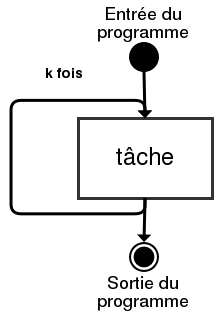
\includegraphics[height=5cm]{img/algoseq.png}}
	  \hspace{5pt}
	  \subfloat[Programme parallèle.]{\label{fig:algoparal}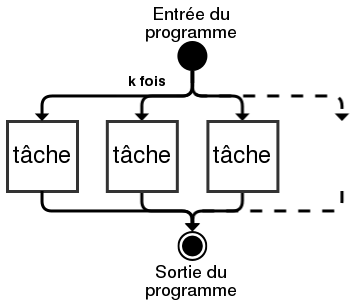
\includegraphics[height=5cm]{img/algoparal.png}}
		\caption[Comparaison du fil d'exécution en séquentiel et parallèle]{Comparaison du fil d'exécution entre un algorithme séquentiel et parallèle. Le temps d'exécution d'un tel algorithme séquentiel (alg\ref{algo:boucletab}) est d'environ $k\times1\,s$ alors que celui d'un algorithme parallèle (alg\ref{algo:paraltab}) est théoriquement de $1\,s$.}
		\label{fig:algoparsec}
	\end{figure}

Le gain en temps de la parallélisation n'est pas négligeable, mais il est impossible de prévoir le temps d'exécution de l'algorithme représenté par la figure~\ref{fig:algoparsec}\subref{fig:algoparal}. En effet les tâches entrent en concurrence et se ralentissent les unes les autres. En théorie, si le nombre d'unités de calcul est suffisant, le temps d'exécution est de 1\,s plus le temps de transfert des données de l'unité mère, créant tous ces fils d'exécution, et les unités filles, celles effectuant le calcul. Dans la pratique ce nombre est limité, c'est pour cela que le nombre de fils d'exécution (\emph{thread}) est modulé par le nombre de processeurs, le nombre de c\oe{}urs, le quota du nombre de processus mis à disposition.

\

On remarque de par la différence de structure de code des algorithmes~\ref{algo:boucletab}~et~\ref{algo:paraltab} que le travaille du programmeur n'est pas le même. La parallélisation a un coût de programmation plus élevé. Il existe deux types de parallélisation, une première appelée \emph{multiprocessing} et une deuxième appelée \emph{multithreading}. Les deux présentent leurs avantages et leurs inconvénients aussi bien au niveau de la programmation que du temps d'exécution. Par simplification une partie de la parallélisation a été effectuée à l'aide d'outils présents au \CC, en particulier \texttt{qsub}.

			\paragraph{\emph{multiprocessing}}
Le \emph{multiprocessing} consiste à lancer un processus différent pour chaque nouveau fil d'exécution. Cela revient à lancer plusieurs fois le même programme mais sur des données différentes. Par la suite le processus mère récupère toutes les données générées par les processus fils crées, et continue son exécution.

Cette technique permet d'avoir une véritable parallélisation puisque les processus créés tournent sur d'autres unités de calcul sans interférence avec le processus mère. Les problèmes possibles sont causés par le système d'exploitation puisque ce dernier possède un ordonnanceur indiquant la liste des processus en exécution, et donne plus ou moins de temps à la fois à chacun. Si trop de processus sont créés, ils ne tourneront que très peu et satureront le quota du nombre de processus autorisés par l'utilisateur.

Cette méthode de parallélisation nécessite simplement différentes unités de calcul indépendantes les unes des autres, de préférence proches physiquement (processeur multi-c\oe{}urs) ; c'est pour cela qu'elle est la plus ancienne car déjà utilisée sur des supercalculateurs comme CRAY~X-MP en 1982.

Cette technique ne sera utilisée que par le biais de \texttt{qsub}.

			\paragraph{\emph{multiprocessing}}
Le \emph{multiprocessing} consiste à exécuter plusieurs \emph{threads} sur une même unité de calcul en utilisant au maximum les ressources disponibles par un c\oe{}ur de processeur, cela demande une architecture particulière. Les \emph{treads} ainsi lancés s'exécutent à des moments différents, le processeur change le \emph{thread} actif à chaque cycle d'horloge. L'architecture des processeurs superscalaires ou vectoriels permet d'exécuter simultanément plusieurs \emph{threads}.

\

Le fait d'exécuter à chaque cycle d'horloge un \emph{thread} différent ne semble pas permettre, à première vue, de gagner en temps d'exécution, mais cela tir partie du fait que le processeur reste inactif la majeure partie du temps car le \emph{thread} actif écrit ou lit de la mémoire plus lente que les registres (RAM).

\

Cette technique n'a été utilisé que pour la récupération des données en effectuant la lecture simultanée de plusieurs fichiers \texttt{fits} et l'envoi de plusieurs requêtes SQL et a donc été utilisée avec le module \Python{} \texttt{multiprocessing} qui implémente le \emph{multiprocessing} et \emph{multithreading}.

		\subsubsection{Envoi des \emph{jobs} avec \texttt{qsub}}
		%^^^^^^^^^^^^^^^^^^^^^^^^^^^^^^^^^^^^^^^^^^^^^^^^^^^^^^^^

La commande \texttt{qsub} est l'ordonnanceur du système \emph{Sun Grid Engine} développé par l'entreprise Sun Microsystems. Cet outil permet de soumettre une tâche, un \emph{job}, sur une machine de \emph{batch}. L'utilisateur n'a accès qu'aux options de soumission de \emph{jobs} et reçoit à fin de l'exécution du programme une paire de fichiers, un pour la sortie standard et un second pour la sortie d'erreurs.

\

L'envoi de \emph{jobs} à l'ordonnanceur s'effectue via une commande du type :
	\begin{verbatim}
		$ qsub -pe multicores 6 -q mc_medium -t 1-10 job.csh
	\end{verbatim} %$
Ceci permet l'exécution du script \texttt{job.csh} qui est un script en \emph{C-shell}, ce qui est préconisé par l'environnement de travail du \CC{}\footnote{Le \emph{shell} par défaut au \CC{} est pour le moment le \texttt{csh}, mais une réflexion est en cours pour changer pour un environnement en \texttt{bash}, \emph{shell} par défaut de nombreux système GNU/Linux et UNIX.}. Ce script permet l'exécution de notre programme écrit en \Python{} et \Cpp{}.

\

Détaillons cette ligne d'exécution qui est déjà réduite au minimum qui nous intéresse.

L'option \texttt{-pe} permet d'indiquer que l'on souhaite utiliser du \texttt{multicores} et d'en disposer de 6. Cette option est utilisée pour le \emph{multithreading} qui s'effectue sur plusieurs c\oe{}urs.

L'option \texttt{-q} permet d'indiquer le nom d'une queue de calcul. Lors de la soumission du \emph{job} avec \texttt{qsub}, notre tâche est placée dans une file d'attente, plusieurs files existent et correspondent chacune à un besoin particulier.

Enfin l'option \texttt{-t} permet d'indiquer à \texttt{qsub} que l'on souhaite envoyer un tableau de \emph{jobs}, cela correspond à l'implémentation du \emph{multiprocessing}. L'option de \texttt{qsub} ne permet pas d'utiliser toute la puissance du \emph{multiprocessing} implémenté dans des bibliothèques standards tels que \texttt{OpenMP}, en effet le dialogue inter-processus n'est pas possible avec \texttt{qsub}. Cependant, dans notre cas, cette possibilité ne présentait pas d'intérêt, il a donc été privilégié d'utiliser des outils déjà existants. Dans cet exemple dix \emph{jobs} seront envoyés et recevront une variable d'environnement \texttt{\$SGE\_TASK\_ID} ayant pour valeur leur indice dans le tableau.

Puis suit le nom du script à exécuter.

		\subsubsection{Script \texttt{init.py}}
		%^^^^^^^^^^^^^^^^^^^^^^^^^^^^^^^^^^^^^^

Pour simplifier l'utilisation du programme et le lancement automatique d'un tableau de \emph{jobs} avec \texttt{qsub} il a été décidé de créer un script d'initialisation. Celui-ci s'inspire d'une partie d'\emph{autotools} en générant les fichiers \texttt{config.h} des différentes parties écrites en \Cpp{} \cite{AUTOTOOLS}. Ceci présente l'avantage de n'avoir qu'un seul fichier de configuration, général à toutes les parties aussi bien \Python{} que \Cpp{}, simple d'écriture, qui est lu par le script \texttt{init.py} pour répartir les informations utiles à chacune des parties, celles-ci étant parfois communes mais ne portant pas les mêmes noms au sein des modules puisque faisant partie de la sortie d'un module, puis de l'entrée du module suivant. La figure~\ref{fig:autotools} résume l'arbre d'organisation d'\emph{autotools}.

	\begin{figure}[h]
		\centering
		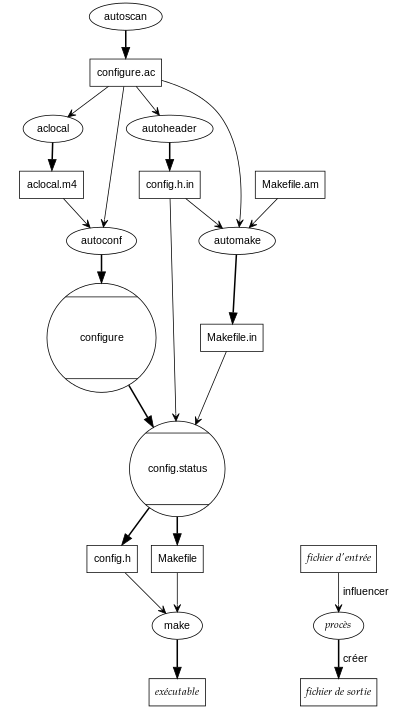
\includegraphics[height=0.6\textheight]{img/autotools.png}
		\caption[Organisation des outils d'\emph{autotools}]{Organisation des différents outils intégrés dans \emph{autotools}, permettant la génération des outils de compilation comme \texttt{Makefile} et la vérification de dépendances pour l'installation de programmes.}
		\label{fig:autotools}
	\end{figure}

	\begin{figure}[h]
		\centering
		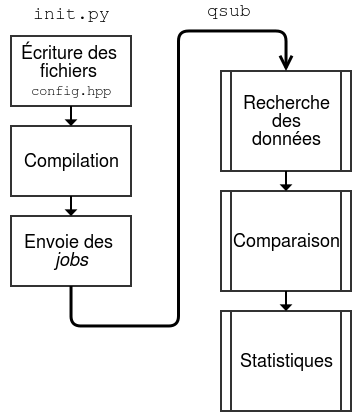
\includegraphics[width=0.4\textwidth]{img/init.png}
		\caption[Instructions effectuées par \texttt{init.py}]{Liste des instructions effectuées par \texttt{init.py} et celles engendrées par son lancement.}
		\label{fig:init}
	\end{figure}

La suite d'instruction de \texttt{init.py} est décrite par la figure~\ref{fig:init}. Cela se divise en trois étapes, tout d'abord l'écriture des fichiers de configuration des modules \Cpp, puis la compilation de celles-ci à l'aide de fichiers \texttt{Makefile} \cite{MAKE}. Avant d'effectuer l'appel à \texttt{qsub}, le script \texttt{init.py} génère un script \texttt{job.py} en \Python{} dont le rôle sera de lancer successivement les différentes tâches demandées ; en effet en argument de l'exécution de \texttt{init.py} il est possible d'indiquer la suite d'exécution des tâches, \texttt{d} pour la recherche des données, \texttt{c} pour la comparaison et \texttt{s} pour la partie statistique, ainsi l'utilisateur final de ce script peut indiquer les tâches qu'il souhaite lancer. Dans la pratique cela a beaucoup servi au débugage et au test des modules indépendamment des autres. Ainsi \texttt{init.py} lance avec \texttt{qsub} le script \texttt{job.py} qui effectuera les appels aux différents modules.


\section{Étude de la stabilité}
%==============================

Pour évaluer la qualité des produits du \stack{} il est intéressant d'observer comment il réagit face à des images de la même région à des instants $t$ distincts. En effet les différentes \emph{runs} effectuées par SDSS sur la \emph{stripe 82} se recouvrent, et donnent lieu à des régions du ciel observées à plusieurs reprises. SDSS est un télescope de surveillance du ciel, il est donc indispensable d'effectuer ces recouvrements, les missions d'observations doivent donc trouver un compromis entre la plus grande couverture du ciel et le meilleur recouvrement.

\

L'intérêt de cette évaluation est de vérifier si le calcul de magnitude par le \stack{} est le même quelles que soient la qualité et la calibration de l'image d'entrée.

	\subsection{Différence entre objet et source}
	%--------------------------------------------

Il est important dans cette partie de distinguer un objet d'une source. L'objet fait référence à l'astre que l'on observe dans le ciel dont données astrophysiques sont connus. Celles-ci inclus les coordonnées, la magnitude, la variation de la magnitude, ainsi que la parallaxe qui correspond au changement de coordonnées dû à la rotation de la Terre autour du Soleil.

La source quant à elle ne correspond qu'à l'image à un instant $t$ d'un objet. Les sources sont les éléments listés par le \stack{}, de même la base de données de SDSS est un catalogue de sources et non d'objets.

\

L'étude de la stabilité s'effectue en sélectionnant un objet astronomique, de préférence une étoile, et en recherchant la liste des sources correspondant à cet astre. Ensuite on regarde les paramètres astrométriques et photométriques des sources ainsi listées. Cette opération peut avoir pour but de créer un catalogue d'objets s'il est effectué sur toutes les sources identifiées par le \stack{}.


	\subsection{Densité d'images}
	%----------------------------

Pour lister les sources correspondant à l'observation d'un objet il est nécessaire de lister les fichiers à travers les différentes \emph{runs} correspondant à cette zone du ciel. Donc la première partie de cette étude fut de parcourir les 16\,000 fichiers \texttt{fits} et de mesurer la densité d'images sur le fond de ciel ainsi que lister les fichiers correspondant à chacune des régions.

	\begin{figure}[h]
		\centering
		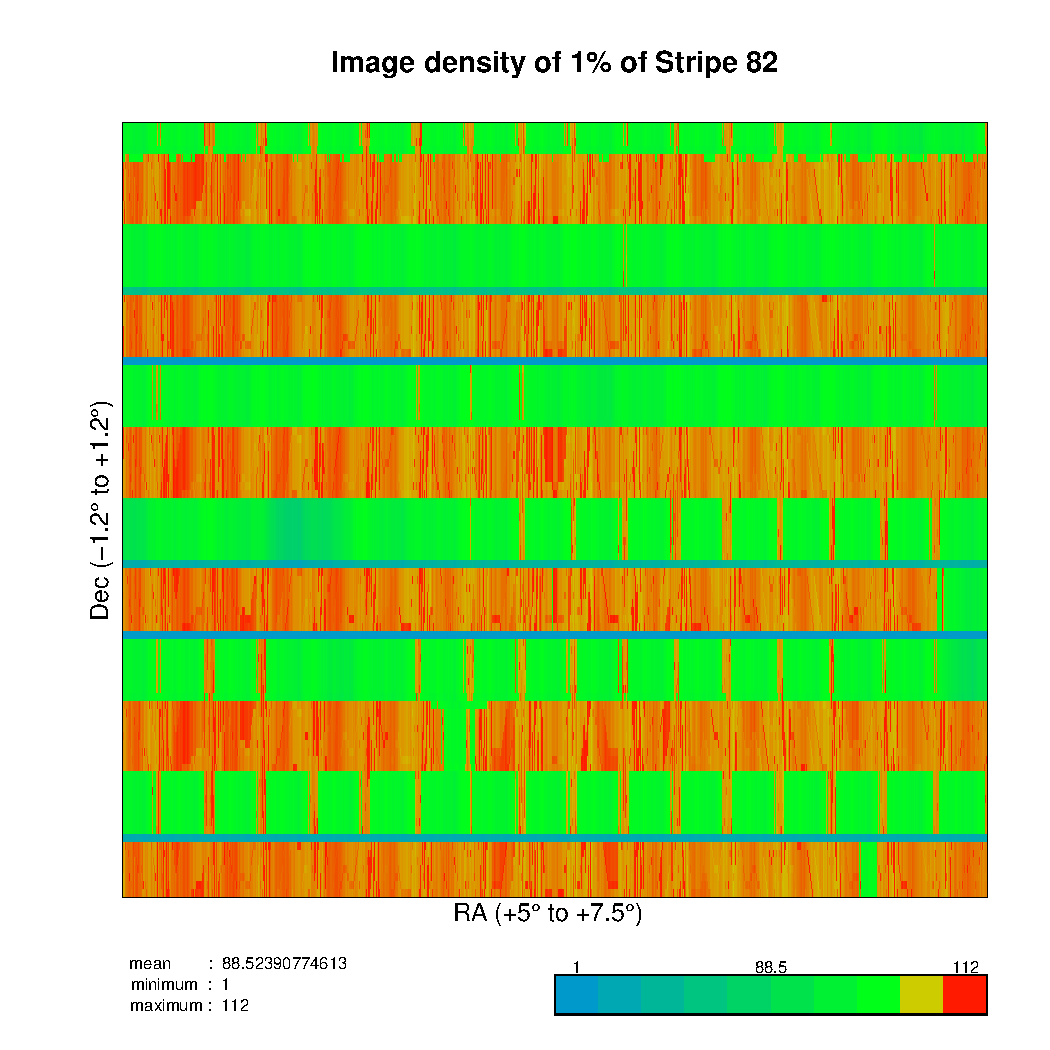
\includegraphics[width=0.8\textwidth]{img/raw/density_one_percent.pdf}
		\caption[Densité d'images de la \emph{stripe 82}]{Densité d'image des 1\% de données de la \emph{stripe 82}.}
		\label{fig:dstrip82}
	\end{figure}

\

La figure~\ref{fig:dstrip82} représente la densité d'images prises par SDSS, qui a été calculée à partir d'un script réalisé en \Python{} ; en effet ce script a vocation à n'être lancé une fois, donc le temps de développement est à prendre en compte dans le temps d'obtention des résultats ; il n'est donc pas indispensable d'avoir un script dont le temps de calcul est le plus faible possible.

Dans ce cas le script parcourt la liste des fichiers pour en récupérer les données intéressantes en 40 minutes. Les données intéressantes sont les indices dans la matrice (une simple conversion des données permet de passer des indices aux coordonnées astronomiques), la densité d'images pour ce coefficient de la matrice ainsi que la liste des fichiers \texttt{fits} associés à cette région du ciel.

\

Pour trouver la liste des fichiers couvrant une zone du ciel, il suffit donc de connaître les coordonnées de la matrice.


	\subsection{Suivi d'un objet}
	%----------------------------

Le suivi d'un objet ne peut se faire qu'une fois la première étape réalisée. Le problème majeur que l'on rencontre est qu'il n'existe pas de catalogue d'objets de si faibles magnitudes. En effet les sources répertoriées par SDSS et le \stack{} sont de magnitude 16 à 23, par comparaison la magnitude limite observable par l'homme est de 6. On rappelle que la magnitude est une échelle logarithmique inverse, donc plus la magnitude est élevée moins l'astre est brillant.

Cette étape effectue donc implicitement la création d'un objet à partir des sources identifiées par le \stack{}, l'objet devant être suivi n'étant pas répertorié.

		\subsubsection{Suivi à partir d'objets d'une autre base}
		%^^^^^^^^^^^^^^^^^^^^^^^^^^^^^^^^^^^^^^^^^^^^^^^^^^^^^^^

Dans un premier temps, il fut imaginé d'utiliser les résultats de l'étape de comparaison pour effectuer ce suivi. Mais l'absence d'objet dans la base de données SDSS ne permit pas d'effectuer cette association objet -- sources.

Il a été envisagé d'effectuer le suivi à partir de sources d'une autre base, comme la base Simbad, base française de l'observatoire de Starsbourg. Cette option demande une nouvelle étape d'association. Le problème rencontré avec cette idée est que la base Simbad comporte encore assez peu d'objets de la magnitude souhaitée.

Le suivi à partir d'une autre base a donc été abandonné car il n'existe pas encore à l'heure actuelle de base convenant pour ce type de comparaison.

		\subsubsection{Suivi à partir de la base du \stack{}}
		%^^^^^^^^^^^^^^^^^^^^^^^^^^^^^^^^^^^^^^^^^^^^^^^^^^^^

Avec l'absence de ressources suffisantes il a été nécessaire de créer une base d'objets pour effectuer ce suivi. Le travail demandé est d'effectuer ce suivi sur un nombre très restreint d'objets, la création d'un catalogue complet n'est pas nécessaire. La procédure pour effectuer ce suivi est d'abord de sélectionner une source dans une zone de très forte densité observée dans l'étape de mesure de la densité dans la région des 1\% de la \emph{stripe 82}. Cette source sera considérée comme notre objet de référence pour le suivi.

L'étape suivante est de relancer l'étape de comparaison, avec des critères de précison plus importants (diminution de la taille de la fenêtre), sur chacun des 112 recouvrements. La comparaison s'effectura essentiellement avec des critères astrométriques car l'erreur due à la photométrie est souvent trop importante à cause de la précision de la calibration, la qualité du ciel au moment de la prise de vue, etc.

Une fois la liste des sources répertoriées correspondant au même objet, nous traçons un graphe de l'évolution des paramètres astrométriques et photométriques.

\

Au moment de l'écriture de ce rapport, cette étude n'est pas encore réalisée.
